\section{A bit more context}

\begin{frame}{A picture of the the Dartmouth workshop}
  \note{
    \begin{itemize}
    \item This is equivalent to the famous photo of the Solvay conference
    \end{itemize}
  }

  \begin{textblock}{90}(5, 10)
    \begin{center}
      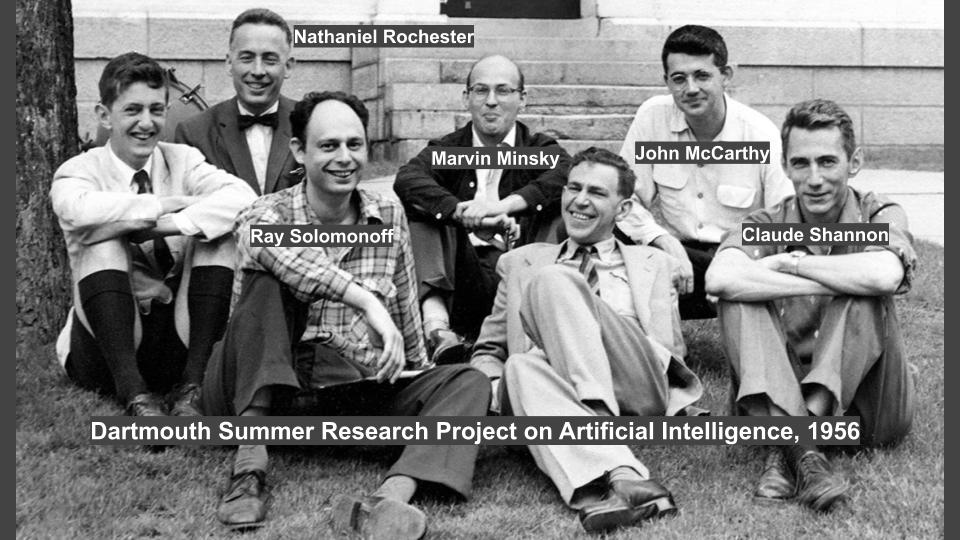
\includegraphics[height=4cm]{img/dartmouth-conference.jpg}
    \end{center}
  \end{textblock}

  \begin{textblock}{95}(5, 58)
    More or less full list of attendees:
    \begin{footnotesize}
    \begin{columns}[T]
      \begin{column}{0.33\textwidth}
        \begin{itemize}
        \item Ray Solomonoff
        \item Marvin Minsky
        \item John McCarthy
        \item Claude Shannon
        \item Trenchard More
        \item Nat Rochester
        \end{itemize}
      \end{column}

      \begin{column}{0.33\textwidth}
        \begin{itemize}
        \item Oliver Selfridge
        \item Julian Bigelow
        \item W. Ross Ashby
        \item W.S. McCulloch
        \item Abraham Robinson
        \item Tom Etter
        \end{itemize}
      \end{column}

      \begin{column}{0.33\textwidth}
        \begin{itemize}
        \item John Nash
        \item David Sayre
        \item Arthur Samuel
        \item Kenneth R. Shoulders
        \item Alex Bernstein
        \item Herbert Simon
        \item Allen Newell
        \end{itemize}
      \end{column}
    \end{columns}
  \end{footnotesize}
\end{textblock}
\end{frame}


% Present the important steps in a project
% Inspired by barra2006, chapter 2, section 1
\begin{frame}
  \frametitle{Steps in a \ac{ML} project}

  \begin{textblock}{90}(5, 15)
    \begin{enumerate}
      % 1.1.1 and 1.1.3
    \item Get familiar with the application domain and the type of data
      % 1.1.2
    \item Get the data and clarify input \& output of each step
      % 1.1.4
    \item Clean and normalize the data
      % 1.1.5
    \item Explore data:
      \begin{itemize}
      \item Descriptive statistics
      \item Visualization
      \end{itemize}
      % 1.1.7 (and 1.1.6)
    \item Compare various methods:
      \begin{itemize}
      \item Take into account the technical limits (computational power \&
        storage, \etc{})
      \item Establish a baseline (``classic method'') and compare other methods
        to it
      \end{itemize}
      % 1.1.8 and 1.1.9
    \item Optimize and evaluate the method
    \item Deploy \& monitor the solution:
      \begin{itemize}
      \item Might require a different implementation to face run time constraints
      \end{itemize}
    \end{enumerate}
  \end{textblock}
\end{frame}
